\section{Systemtest med bruger-input}

\subsection{Beskrivelse}
For at teste det samlede system med bruger-input påsættes den positive og den negative elektrode på rectus femoris, og referenceelektroden påsættes anklen, som illustreret i \autoref{sec:pilotforsoeg} på henholdsvis \autoref{fig:laarmuskler} og \autoref{fig:reference}, ud fra SENIAMs anvisninger \citep{seniam2016}. Huden præpareres inden for at fjerne hår og døde hudceller. 
De to accelerometre påsættes breadboards for at stabilisere deres placering. Disse placeres parallelt med femur og parallelt med tibia, hvilket er illustreret på \autoref{fig:accelerometervinkel}.

Systemet testes over 10 sekunders måling, hvilket samples via mikrokontrolleren. Der skal hertil foretages to målinger, hvor forsøgspersonen starter med at stå oprejst og overskride en vinkel på 180$^{\circ}$ af knæet ved at overstrække knæleddet. Herefter udfører forsøgspersonen en squat-øvelse, hvilket får vinklen af knæet til at overskride grænsen på $90^{\circ}$. Forsøgspersonen bevæger sig herefter tilbage til udgangsposition, hvor de 180$^{\circ}$ overskrides ved overstræk af knæleddet.
På denne måde testes det, hvorvidt det samlede system fungerer, da en overskridelse af intervallet $90-180^{\circ}$ vil betyde, at data ikke bliver behandlet i EMG-algoritmen. Dette illustreres ved, at det digitale output er 0. Under testen opsamles det samplede digitalt filtrede EMG-signal, EMG-algoritmen og vinklen over knæet.

\subsection{Resultater af forsøg}

På \autoref{fig:test_squat} ses en illustration af systemet påsat forsøgspersonen, og mikrokontrolleren ses koblet til forsøgspersonen.

\begin{figure}[H]
\centering
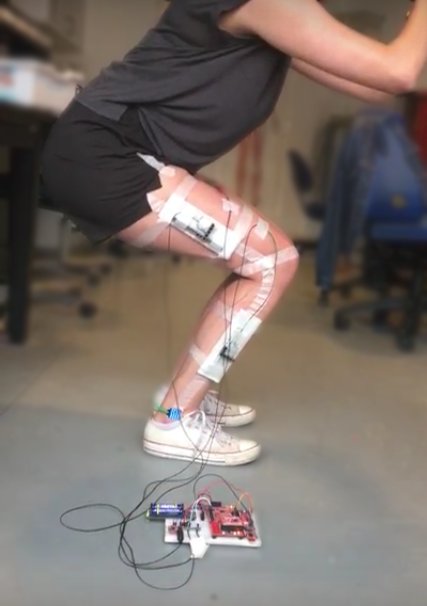
\includegraphics[width=0.7\textwidth]{figures/test_squat}
\caption{Forsøgsopstilling til udførelse af systemtest med bruger-input. Forsøgspersonen er her på vej ned i squat-øvelsen.}
\label{fig:test_squat}
\end{figure}

\noindent
På baggrund af testen er systemets input samt output plottet og visualiseret. Visualisering af de opsamlede signaler forekommer af \autoref{fig:test_brugerinput}. 

\begin{figure}[H]
\centering
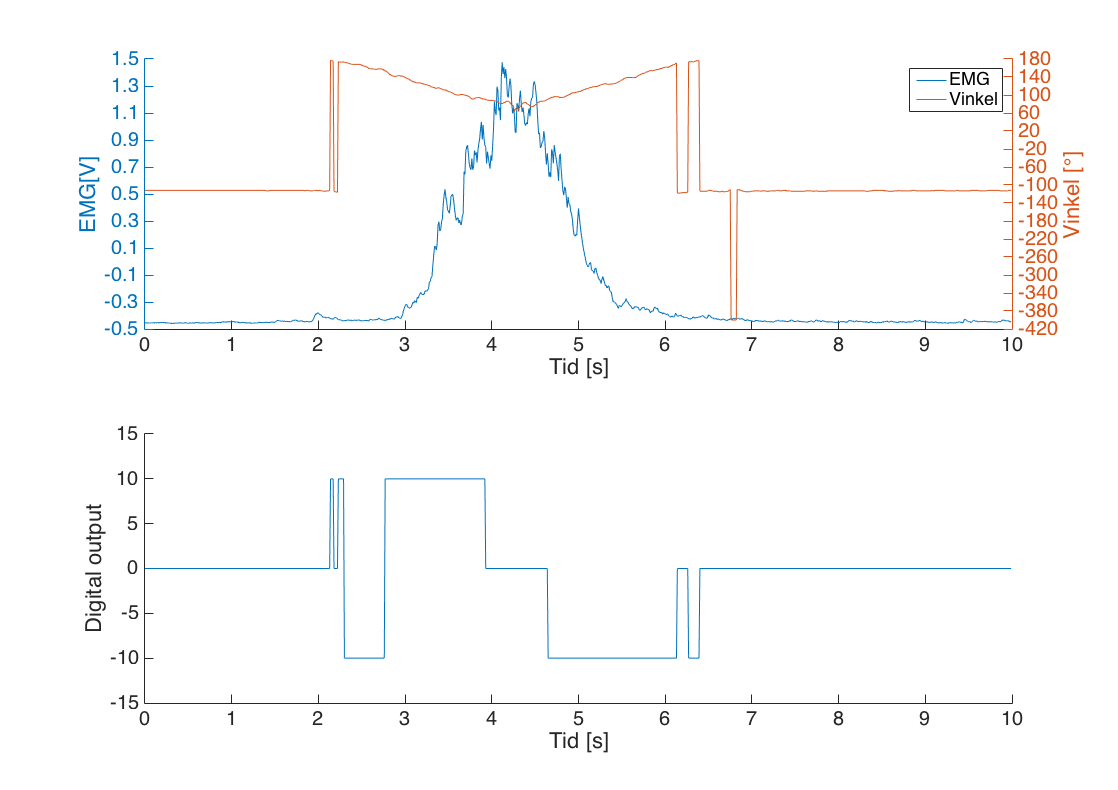
\includegraphics[width=1\textwidth]{figures/test_brugerinput}
\caption{På den øverste graf ses muskelaktivitet ved udførelse af en squat-øvelse samt vinklen over knæet under øvelsen. Den blå graf illustrerer det samplede digital filtrerede EMG og den røde graf illustrerer vinklen over knæet. Hertil ses et fald til under $-100^{\circ}$, hvilket illustrerer en overskridelse af $180^{\circ}$. Den nederste graf illusterer signalets digitale output i EMG-algoritmen. Denne visualiserer en stigning og et fald af det opsamlede EMG-signal, hvorved en stigning af muskelaktiviteten illustreres som værende $+10$ og et fald i muskelaktiviteten som værende $-10$. Ved grafen lig 0 illustreres en overskridelse af $90-180^{\circ}$ af knæet.}
\label{fig:test_brugerinput}
\end{figure}

\noindent
Ud fra \autoref{fig:test_brugerinput} ses en sammenhæng mellem muskelaktiviteten under en squat-øvelse og vinklen over knæet under øvelsen. Ved en stigning af muskelaktiviteten ses et fald i vinklen over knæet, hvilket sker mellem $2-4~s$. Ved fald i muskelaktivitet stiger vinklen over knæet, hvilket ses mellem $4,5-6,5~s$.
Ved starten af testen overstrækker forsøgspersonen knæet, hvilket ses ved, at vinklen er $-112^{\circ}$. 

Grunden til at vinklen er $-112^{\circ}$ og ikke $-400^{\circ}$ er, at det ene accelerometer har været indenfor grænsen på $180^{\circ}$ og det andet accelerometer har overskredet grænsen. Det ene accelerometer har derfor haft en vinkel på $88^{\circ}$, mens det andet accelerometer har overskredet dens grænse, hvorfor den samlede vinkel er $-112^{\circ}$. Det samme gør sig gældende ved slutningen af øvelsen. Ved overstrækning af knæet, og dermed overskridelse af $180^{\circ}$, ses EMG-algoritmens output som værende 0. 
Efter $2~s$ overstrækkes knæet ikke længere og graderne begynder derved at falde i takt med, at muskelaktiviteten stiger. 

Ved en stigning af muskelaktiviteten ses EMG-algoritmen ligeledes stigende. Ved $4~s$ er vinklen over knæet $81^{\circ}$, hvilket er en overskridelse af grænsen på $90^{\circ}$. Dette illustreres ved, at EMG-algoritmens output er 0. 
Efter $4,5~s$ ses en stigning af vinklen i takt med et fald i muskelaktiviteten. Derved ses ligeledes et fald i EMG-algoritmens output. 
Efter $6~s$ overstrækkes knæet igen, hvorefter begge accelerometre overskrider deres grænser, hvorfor grafen illustrerer $-400^{\circ}$. Herefter overstrækkes knæene fortsat, dog ligger det ene accelerometer indenfor dens grænse, hvilket forklarer vinklen på $-112^{\circ}$. 
